
\begin{center}
\begin{LARGE}
\textbf{Supplementary Information}
\end{LARGE}\\
Alberto Scarampi (as2945@cam.ac.uk)\\
January 2021 
\end{center}

\section{Extended Methods on CyanoGate Assembly}
\label{sec:cyanogate}
All the plasmids generated in this study were assembled using Golden Gate, a DNA assembly method that employs Type-IIS restriction enzymes to cut DNA sequences at specific locations and T4 DNA ligase to paste different fragments together. Type-IIS restriction enzymes (BbsI, BsaI) cut DNA at locations outside of their hexameric recognition sequences  (e.g. GAAGAC for BBsI) and generate 4-bp long single-stranded overhangs. By designing complementary sets of overhang sequences and assigning standardised overhang to different types DNA parts (e.g. promoters, coding sequences etc...) modular cloning systems (MoClo) have been developed \citep{Weber2011}. MoClo systems are available for various synthetic biology chassis and enable a rapid and easy-to-share method to construct modular DNA libraries without proprietary tools and reagents \citep{Patron2015}.The MoClo syntax is also seen as the most suitable assembly standard for automated synthesis in DNA Foundries \citep{Chambers2016}.
For these reasons a MoClo toolbox developed for synthetic biology in cyanobacteria (CyanoGate) was used in this project. This is derived from the MoClo system for plants and microalgae (\citealt{Engler2014}; \citealt{Crozet2018}), and has been adopted by various open-source synthetic biology initiatives (\href{https://www.openplant.org/}{OpenPlant}, \href{http://parts.igem.org/Main_Page}{iGEM}) \citep{Vasudevan2019}. In order to make the DNA parts compatible with the CyanoGate toolbox,  the genes required in this project were amplified using primers containing part-specific overhangs as listed in Table \ref{table:overhangs}.

\begin{table}[H]
\begin{tabular}{|c|c|c|c|c|}
\hline
\textbf{Part Type} & \textbf{Description} & \textbf{Backbone} & \textbf{Prefix (5'-3')} & \textbf{Suffix (5'-3')} \\ \hline
Prom + 5U & promoter + RBS & pICH41295 & GGAG & AATG \\ \hline
CDS1 & coding sequence (with stop codon) & pICH41308 & AATG & GCTT \\ \hline
Cas12 gRNA & cas12a direct repeat + spacer & pICH42120 & TAGC & TTCG \\ \hline
HDR & homology directed repair template & pICH41331 & GGAG & TCGC \\ \hline
3U + Ter & 3'-UTR / terminator & pICH41276 & GCTT & CGCT \\ \hline
\end{tabular}
\caption{List of parts and overhang standards for MoClo assembly in cyanobacteria.}
\label{table:overhangs}
\end{table}

\subsection{PCR Amplification to Clone Native Genes into L0 Acceptors}
\label{sec:PCR}

The native sequences required for this project (homology repair templates, prqR, prqA) were cloned from genomic DNA extracted from \textit{Synechocystis sp.} PCC 6803. DNA was extracted from a 50 mL culture (grown to stationary phase) using the GeneJET Genomic DNA Purification Kit (Thermo Scientific)  according to the manufacturer instructions.
PCR reactions to amplify native sequence with primers containing MoClo overhangs (as listed in Table \ref{table:overhangs}) were performed using Phusion High-Fidelity Polymerase (ThermoFisher) and were carried out with the reagents listed in Table \ref{table:PCRreagents}.

\begin{table}[H]
\begin{tabular}{|c|c|c|c|}
\hline
\textbf{Component} & \textbf{[Working]} & \textbf{[Stock]} & \multicolumn{1}{l|}{\textbf{Volume to add ($\mu$l per 50 $\mu$l rxn)}} \\ \hline
Autoclaved $H_{2}O$ & 1x & 1x & up to 50 \\ \hline
Phusion HF Buffer & 1x & {\color[HTML]{333333} 5x} & 10 \\ \hline
dNTPs & 200 nM & {\color[HTML]{333333} 10000 nM} & 1 \\ \hline
Genomic DNA & {\color[HTML]{000000} 1 ng} & {\color[HTML]{333333} [nanodrop]} & 50/[nanodrop] \\ \hline
Forward Primer & 0.5 $\mu$M & 25 $\mu$M & 1 \\ \hline
Reverse Primer & 0.5 $\mu$M & 25 $\mu$M & 1 \\ \hline
Phusion$^{TM}$ Polymerase & 0.02 U/$\mu$l & 2 U/$\mu$l & 0.5 \\ \hline
\end{tabular}
\caption{List of reagents and their concentrations used for  PCR reactions}
\label{table:PCRreagents}
\end{table}

PCR reactions were carried out in 0.2 mL tubes in a PCR Thermocycler (Eppendorf). Annealing temperatures (Tm) for each set of primers were calculated with the \href{https://tmcalculator.neb.com/#!/main}{NEB Tm calculator} software using the homologous sequences as input. Cycling conditions are listed in Table \ref{table:cycling}.


\begin{table}[H]
\centering
\begin{tabular}{|l|c|c|c|}
\hline
\textbf{Cycle Step} & \multicolumn{1}{l|}{\textbf{Temp (C)}} & \multicolumn{1}{l|}{\textbf{Time  (s)}} & \multicolumn{1}{l|}{\textbf{Cycles}} \\ \hline
Initial denaturation & 98 & 30 & 1 \\ \hline
Denaturation & 98 & 5-10 sec &  \\ \cline{1-3}
Annealing & {\color[HTML]{D10E0E} \textbf{Tm}} & 10-30 sec &  \\ \cline{1-3}
Extension & 72 & 0.015 sec/bp & \multirow{-3}{*}{25-35} \\ \hline
Final Extension & 72 & 5-10 min & 1 \\ \hline
Hold & 4 & Hold & Hold \\ \hline
\end{tabular}
\caption{Parameters for thermal cycling performed to clone parts into level 0 acceptors.}
\label{table:cycling}
\end{table}

The PCR amplicons were then purified with a PCR Cleanup kit (NEB), digested and ligated in the same tube with acceptor plasmids (2:1 insert:backbone ratio), BbsI and T4 DNA Ligase. Sequences were validated by Sanger sequencing following plasmid extraction from white \textit{E. coli} colonies transformed with the assembly reactions.



\subsection{Oligo Annealing to Clone Short Parts into L0 Acceptors}
\label{sec:Annealing}

Short DNA sequences (e.g. promoters, gRNA) were constructed by annealing synthetic oligonucleotides as described by \citep{Stemmer1995}. For sequences shorter than 50 bp, double-stranded genes were assembled by designing sets of complimentary primers with desired overhangs and annealed by heating at 95$^{\circ}$C and cooling slowly to 4$^{\circ}$C. 
Longer sequences (promoters) or with secondary structures (e.g. terminators) anneal better by designing overlapping primers with 20 bp complementarity and extending them using dNTPs and a DNA polymerase enzyme (e.g. Phusion$^{TM}$) as in a PCR reaction.
\begin{figure}[H]
    \centering
    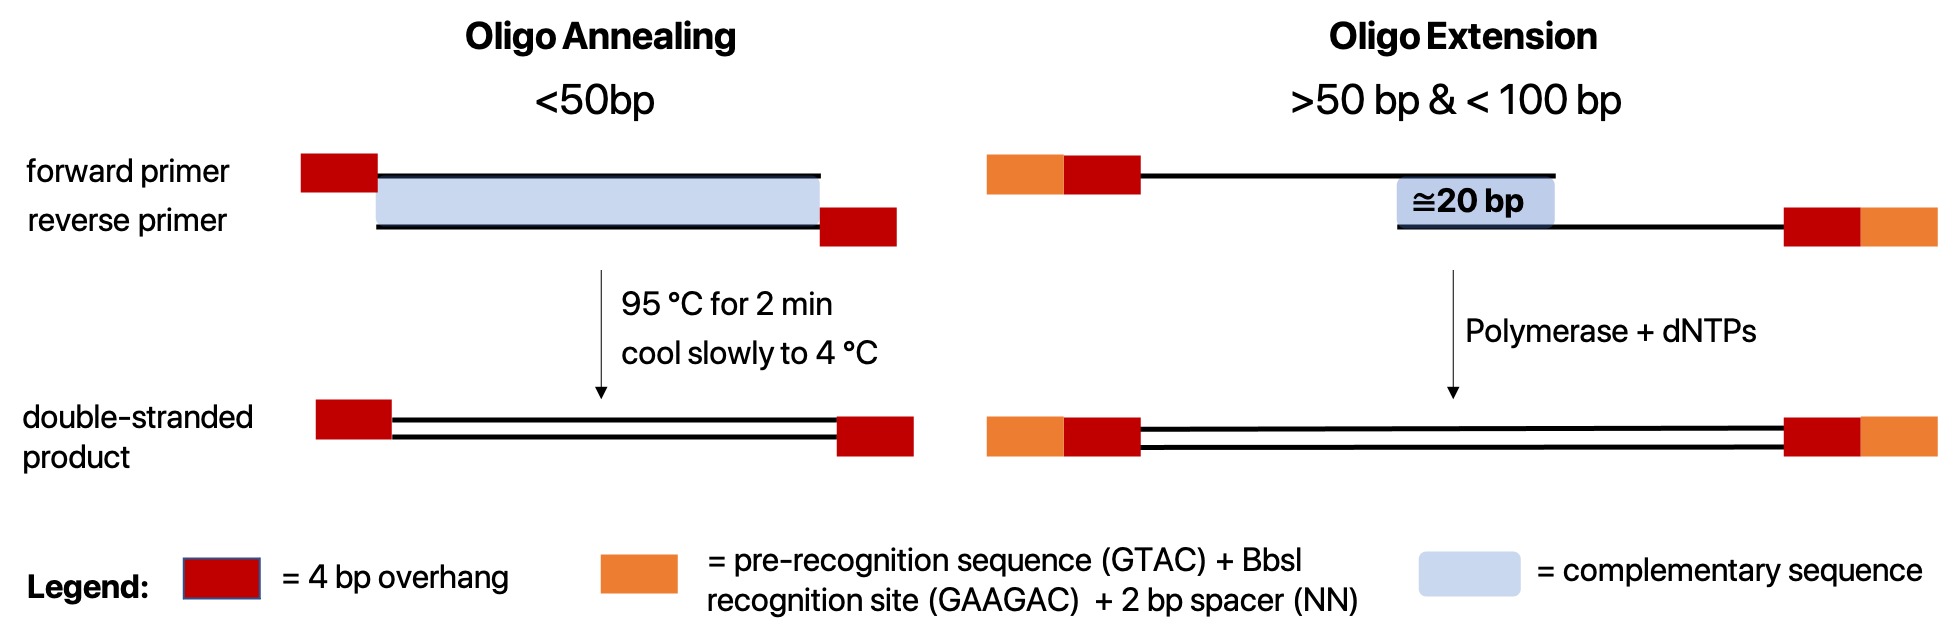
\includegraphics[width=\hsize]{figs/oligos.png}
    \caption{Strategies for annealing and extension of synthetic oligonucleotides}
\end{figure}

For annealing, complementary oligonucleotides were dissolved at a 1:1 molar ratio in an annealing buffer containing 10 mM Tris, 1 mM EDTA, 50 mM NaCl (adjusted to a pH of 8.0). Table \ref{table:annealingpar} lists the reagents and their concentrations used for these reactions.

\begin{table}[H]
\centering
\begin{tabular}{|c|c|c|c|}
\hline
\textbf{Component} & \textbf{[Working]} & \textbf{[Stock]} & \textbf{\textbf{Volume to add ($\mu$l per 50 $\mu$l rxn)}} \\ \hline
Primer F & 2.5 $\mu$M & 25 $\mu$M & 5 \\ \hline
Primer R & 2.5 $\mu$M & 25 $\mu$M & 5 \\ \hline
Annealing buffer & 1x & 10x & 5 \\ \hline
milliQ $H_{2}0$ & 1x & 1x & 35 \\ \hline
\end{tabular}
\caption{List of reagents for annealing single-stranded oligonucleotides}
\label{table:annealingpar}
\end{table}

Oligo extension was performed with the PCR parameters listed in Table \ref{table:PCRreagents} and \ref{table:cycling} with no template DNA (the primers are the template). The melting temperature was calculated using the 20 bp overlap as input in the \href{https://tmcalculator.neb.com/#!/main}{NEB Tm calculator} software.

\begin{table}[H]
\begin{adjustwidth}{-1.5cm}{-1.5cm}
\centering
\begin{tabular}{|c|c|l|c|}
\hline
{\color[HTML]{333333} \textbf{Label}} & {\color[HTML]{333333} \textbf{Primer}} & \multicolumn{1}{c|}{{\color[HTML]{333333} \textbf{DNA Sequence (5'$\rightarrow$3')}}} & {\color[HTML]{333333} \textbf{Used for:}} \\ \hline
{\color[HTML]{333333} P1} & {\color[HTML]{333333} PrqA-1F} & {\color[HTML]{333333} GTACGAAGACct\textbf{AATG}acagatatttcaatgcgatttgg} & {\color[HTML]{333333} L0 PCR} \\ \hline
{\color[HTML]{333333} P2} & {\color[HTML]{333333} PrqA-1R} & {\color[HTML]{333333} GTACGAAGACct\textbf{AAGC}ttaagatctagcaacgggaaggg} & {\color[HTML]{333333} L0 PCR} \\ \hline
{\color[HTML]{333333} P3} & {\color[HTML]{333333} PrqR-part1-1F} & {\color[HTML]{333333} GTACGAAGACct\textbf{AATG}gtttctggaaaaaggcttcgttc} & {\color[HTML]{333333} L0 PCR} \\ \hline
{\color[HTML]{333333} P4} & {\color[HTML]{333333} PrqR-part1-1R} & {\color[HTML]{333333} GTACGAAGACac\textbf{CAGG}ggagcaaaaccgtgtaag} & {\color[HTML]{333333} L0 PCR} \\ \hline
{\color[HTML]{333333} P6} & {\color[HTML]{333333} PrqR-part2-1F} & {\color[HTML]{333333} \begin{tabular}[c]{@{}l@{}}\textbf{CCTG}gaGgaccccctgcgctcccaggtcattgccactgctc\\ tgaaactggcccagctatag\end{tabular}} & {\color[HTML]{333333} annealing} \\ \hline
{\color[HTML]{333333} P7} & {\color[HTML]{333333} PrqR-part2-1R} & {\color[HTML]{333333} \begin{tabular}[c]{@{}l@{}}\textbf{AAGC}ctatagctgggccagtttcagagcagtggcaatgacctg\\ ggagcgcagggggtcttc\end{tabular}} & {\color[HTML]{333333} annealing} \\ \hline
{\color[HTML]{333333} P37} & {\color[HTML]{333333} $\Delta$PrqA-HRT-UP-3F} & {\color[HTML]{333333} GTACGAAGACTC\textbf{GGAG}tttcaatgcgatttggcatgc} & {\color[HTML]{333333} L0 PCR} \\ \hline
{\color[HTML]{333333} P38} & {\color[HTML]{333333} $\Delta$PrqA-HRT-UP-3R} & {\color[HTML]{333333} GTACGAAGACTC\textbf{TCGT}gggttatgaacaacattcccgg} & {\color[HTML]{333333} L0 PCR} \\ \hline
{\color[HTML]{333333} P45} & {\color[HTML]{333333} $\Delta$PrqA-HRT-DOWN-3F} & {\color[HTML]{333333} GTACGAAGACTC\textbf{ACGA}gtattattcatgctgaccgctggc} & {\color[HTML]{333333} L0 PCR} \\ \hline
{\color[HTML]{333333} P40} & {\color[HTML]{333333} $\Delta$PrqA-HRT-DOWN-3R} & {\color[HTML]{333333} GTACGAAGACTC\textbf{AGCG}gccaatgtatgttccgatccaaac} & {\color[HTML]{333333} L0 PCR} \\ \hline
{\color[HTML]{333333} P41} & {\color[HTML]{333333} $\Delta$PrqR-HRT-UP-2F} & {\color[HTML]{333333} GTACGAAGACTC\textbf{GGAG}tgcattatctgcggaggcg} & {\color[HTML]{333333} L0 PCR} \\ \hline
{\color[HTML]{333333} P42} & {\color[HTML]{333333} $\Delta$PrqR-HRT-UP-2R} & {\color[HTML]{333333} GTACGAAGACTC\textbf{AGCC}tccttggtgggaaag} & {\color[HTML]{333333} L0 PCR} \\ \hline
{\color[HTML]{333333} P43} & {\color[HTML]{333333} $\Delta$PrqR-HRT-DOWN-2F} & {\color[HTML]{333333} GTACGAAGACTC\textbf{GGCT}aaactggcccagctatagtttcc} & {\color[HTML]{333333} L0 PCR} \\ \hline
{\color[HTML]{333333} P44} & {\color[HTML]{333333} $\Delta$PrqR-HRT-DOWN-2R} & {\color[HTML]{333333} GTACGAAGACTC\textbf{AGCGa}aattcacgggcctctgct} & {\color[HTML]{333333} L0 PCR} \\ \hline
{\color[HTML]{333333} P10} & {\color[HTML]{333333} $\Delta$PrqRA-HRT-UP1-1F} & {\color[HTML]{333333} GTACGAAGACTC\textbf{GGAG}ctaccaacacaatgccccagagg} & {\color[HTML]{333333} L0 PCR} \\ \hline
{\color[HTML]{333333} P11} & {\color[HTML]{333333} $\Delta$PrqRA-HRT-UP1-1R} & {\color[HTML]{333333} GTACGAAGACTA\textbf{TGGC}gacctggaaataattaaaccgtccagttgg} & {\color[HTML]{333333} L0 PCR} \\ \hline
{\color[HTML]{333333} P12} & {\color[HTML]{333333} $\Delta$PrqRA-HRT-UP2-1F} & {\color[HTML]{333333} \textbf{GCCA}gtcaatttaaaaaagaatatttgcattatctgcggaggcgaaattat} & {\color[HTML]{333333} annealing} \\ \hline
{\color[HTML]{333333} P13} & {\color[HTML]{333333} $\Delta$PrqRA-HRT-UP2-1R} & {\color[HTML]{333333} \begin{tabular}[c]{@{}l@{}}\textbf{AGTC}ATAATTTCGCCTCCGCAGATAATGcaaatat\\ tcttttttaaattgac\end{tabular}} & {\color[HTML]{333333} annealing} \\ \hline
{\color[HTML]{333333} P18} & {\color[HTML]{333333} $\Delta$PrqRA-HRT-DOWN-1F} & {\color[HTML]{333333} GTACGAAGACga\textbf{GACT}cccgttgctagatcttaatccataattgcc} & {\color[HTML]{333333} L0 PCR} \\ \hline
{\color[HTML]{333333} P19} & {\color[HTML]{333333} $\Delta$PrqRA-HRT-DOWN-1F} & {\color[HTML]{333333} GTACGAAGACgc\textbf{AGCG}agggaggagcgttaaagggaac} & {\color[HTML]{333333} L0 PCR} \\ \hline
{\color[HTML]{333333} P54} & {\color[HTML]{333333} PmScarletI-1F} & {\color[HTML]{333333} GTACGAAGACct\textbf{AATG}agtaaaggagaagctgtg} & {\color[HTML]{333333} L0 PCR} \\ \hline
{\color[HTML]{333333} P55} & {\color[HTML]{333333} PmScarletI-1R} & {\color[HTML]{333333} GTACGAAGACct\textbf{AAGC}ttatttgtatagttcatccatgcc} & {\color[HTML]{333333} L0 PCR} \\ \hline
{\color[HTML]{333333} P20} & {\color[HTML]{333333} Cas12a-gRNA-prqR-1F} & {\color[HTML]{333333} \begin{tabular}[c]{@{}l@{}}\textbf{TAGC}TAATTTCTACTAAGTGTAGATtggaaa\\ cattgcatcaggaactt\end{tabular}} & {\color[HTML]{333333} annealing} \\ \hline
{\color[HTML]{333333} P21} & {\color[HTML]{333333} Cas12a-gRNA-prqR-1R} & {\color[HTML]{333333} \begin{tabular}[c]{@{}l@{}}\textbf{AAGC}aagttcctgatgcaatgtttccaATCTACACTT\\ AGTAGAAATTA\end{tabular}} & {\color[HTML]{333333} annealing} \\ \hline
{\color[HTML]{333333} P22} & {\color[HTML]{333333} Cas12a-gRNA-prqA-1F} & {\color[HTML]{333333} \begin{tabular}[c]{@{}l@{}}\textbf{TAGC}TAATTTCTACTAAGTGTAGATagattccta\\ tttgaatgtgatgg\end{tabular}} & {\color[HTML]{333333} annealing} \\ \hline
{\color[HTML]{333333} P23} & {\color[HTML]{333333} Cas12a-gRNA-prqA-1R} & {\color[HTML]{333333} \begin{tabular}[c]{@{}l@{}}\textbf{AAGC}ccatcacattcaaataggaatctATCTACACTTA\\ GTAGAAATTA\end{tabular}} & {\color[HTML]{333333} annealing} \\ \hline
{\color[HTML]{333333} P58} & {\color[HTML]{333333} PprqR-3F} & {\color[HTML]{333333} \begin{tabular}[c]{@{}l@{}}GTACGAAGACCT\textbf{GGAG}gtatcttgaaagtgtccaac\\ caactggacggtttaattatttccaggtcGCc\end{tabular}} & {\color[HTML]{333333} extension} \\ \hline
{\color[HTML]{333333} P59} & {\color[HTML]{333333} PprqR-3R} & {\color[HTML]{333333} \begin{tabular}[c]{@{}l@{}}GTACGAAGACCT\textbf{CATT}ataatttcgcctccgcagata\\ atgcaaatattcttttttaaattgacagGCgacctggaaataattaaaccgtcc\end{tabular}} & {\color[HTML]{333333} extension} \\ \hline
{\color[HTML]{333333} P60} & {\color[HTML]{333333} PprqA-2F} & {\color[HTML]{333333} GTACGAAGACCT\textbf{GGAG}catatttaataactattttagttctttgg} & {\color[HTML]{333333} extension} \\ \hline
{\color[HTML]{333333} P61} & {\color[HTML]{333333} PprqA-2R} & {\color[HTML]{333333} GTACGAAGACCT\textbf{CATT}agcattgacccaaagaactaaaatagttat} & {\color[HTML]{333333} extension} \\ \hline
{\color[HTML]{333333} P62} & {\color[HTML]{333333} TprqR-2F} & {\color[HTML]{333333} \begin{tabular}[c]{@{}l@{}}GTACGAAGACCT\textbf{GCTT}tttcccaatttttcatcttttgc\\ cgacgtttgccaaatggtttccagcgctggttggtggctctaggg\end{tabular}} & {\color[HTML]{333333} extension} \\ \hline
{\color[HTML]{333333} P63} & {\color[HTML]{333333} TprqR-2R} & {\color[HTML]{333333} \begin{tabular}[c]{@{}l@{}}GTACGAAGACCT\textbf{AGCG}aaaaaacaaattttctctaa\\ agatattccctagagccaccaaccagcg\end{tabular}} & {\color[HTML]{333333} extension} \\ \hline
\end{tabular}
\end{adjustwidth}
\captionsetup{width= 7.7in}
\caption{List of oligonucleotide sequences used during this project. Uppercase letters denote overhang sequences (4bp restriction overhangs in bold), lowercase correspond to sequences homologous to genomic loci.}
\label{table:primers}
\end{table}

\subsection{Modular Assembly of CRISPR Knock-Out Plasmids}
The native or synthetic DNA parts assembled as above were used to assemble knock-out plasmids required to generate the $\Delta$prqR, $\Delta$prqA, $\Delta$prqRA mutants. Figure \ref{fig:KOstrategy} illustrates the Golden Gate cloning strategy employed to assemble the level 0 parts into level T knock-out plasmids. 


\begin{figure}[H]
    \centering
    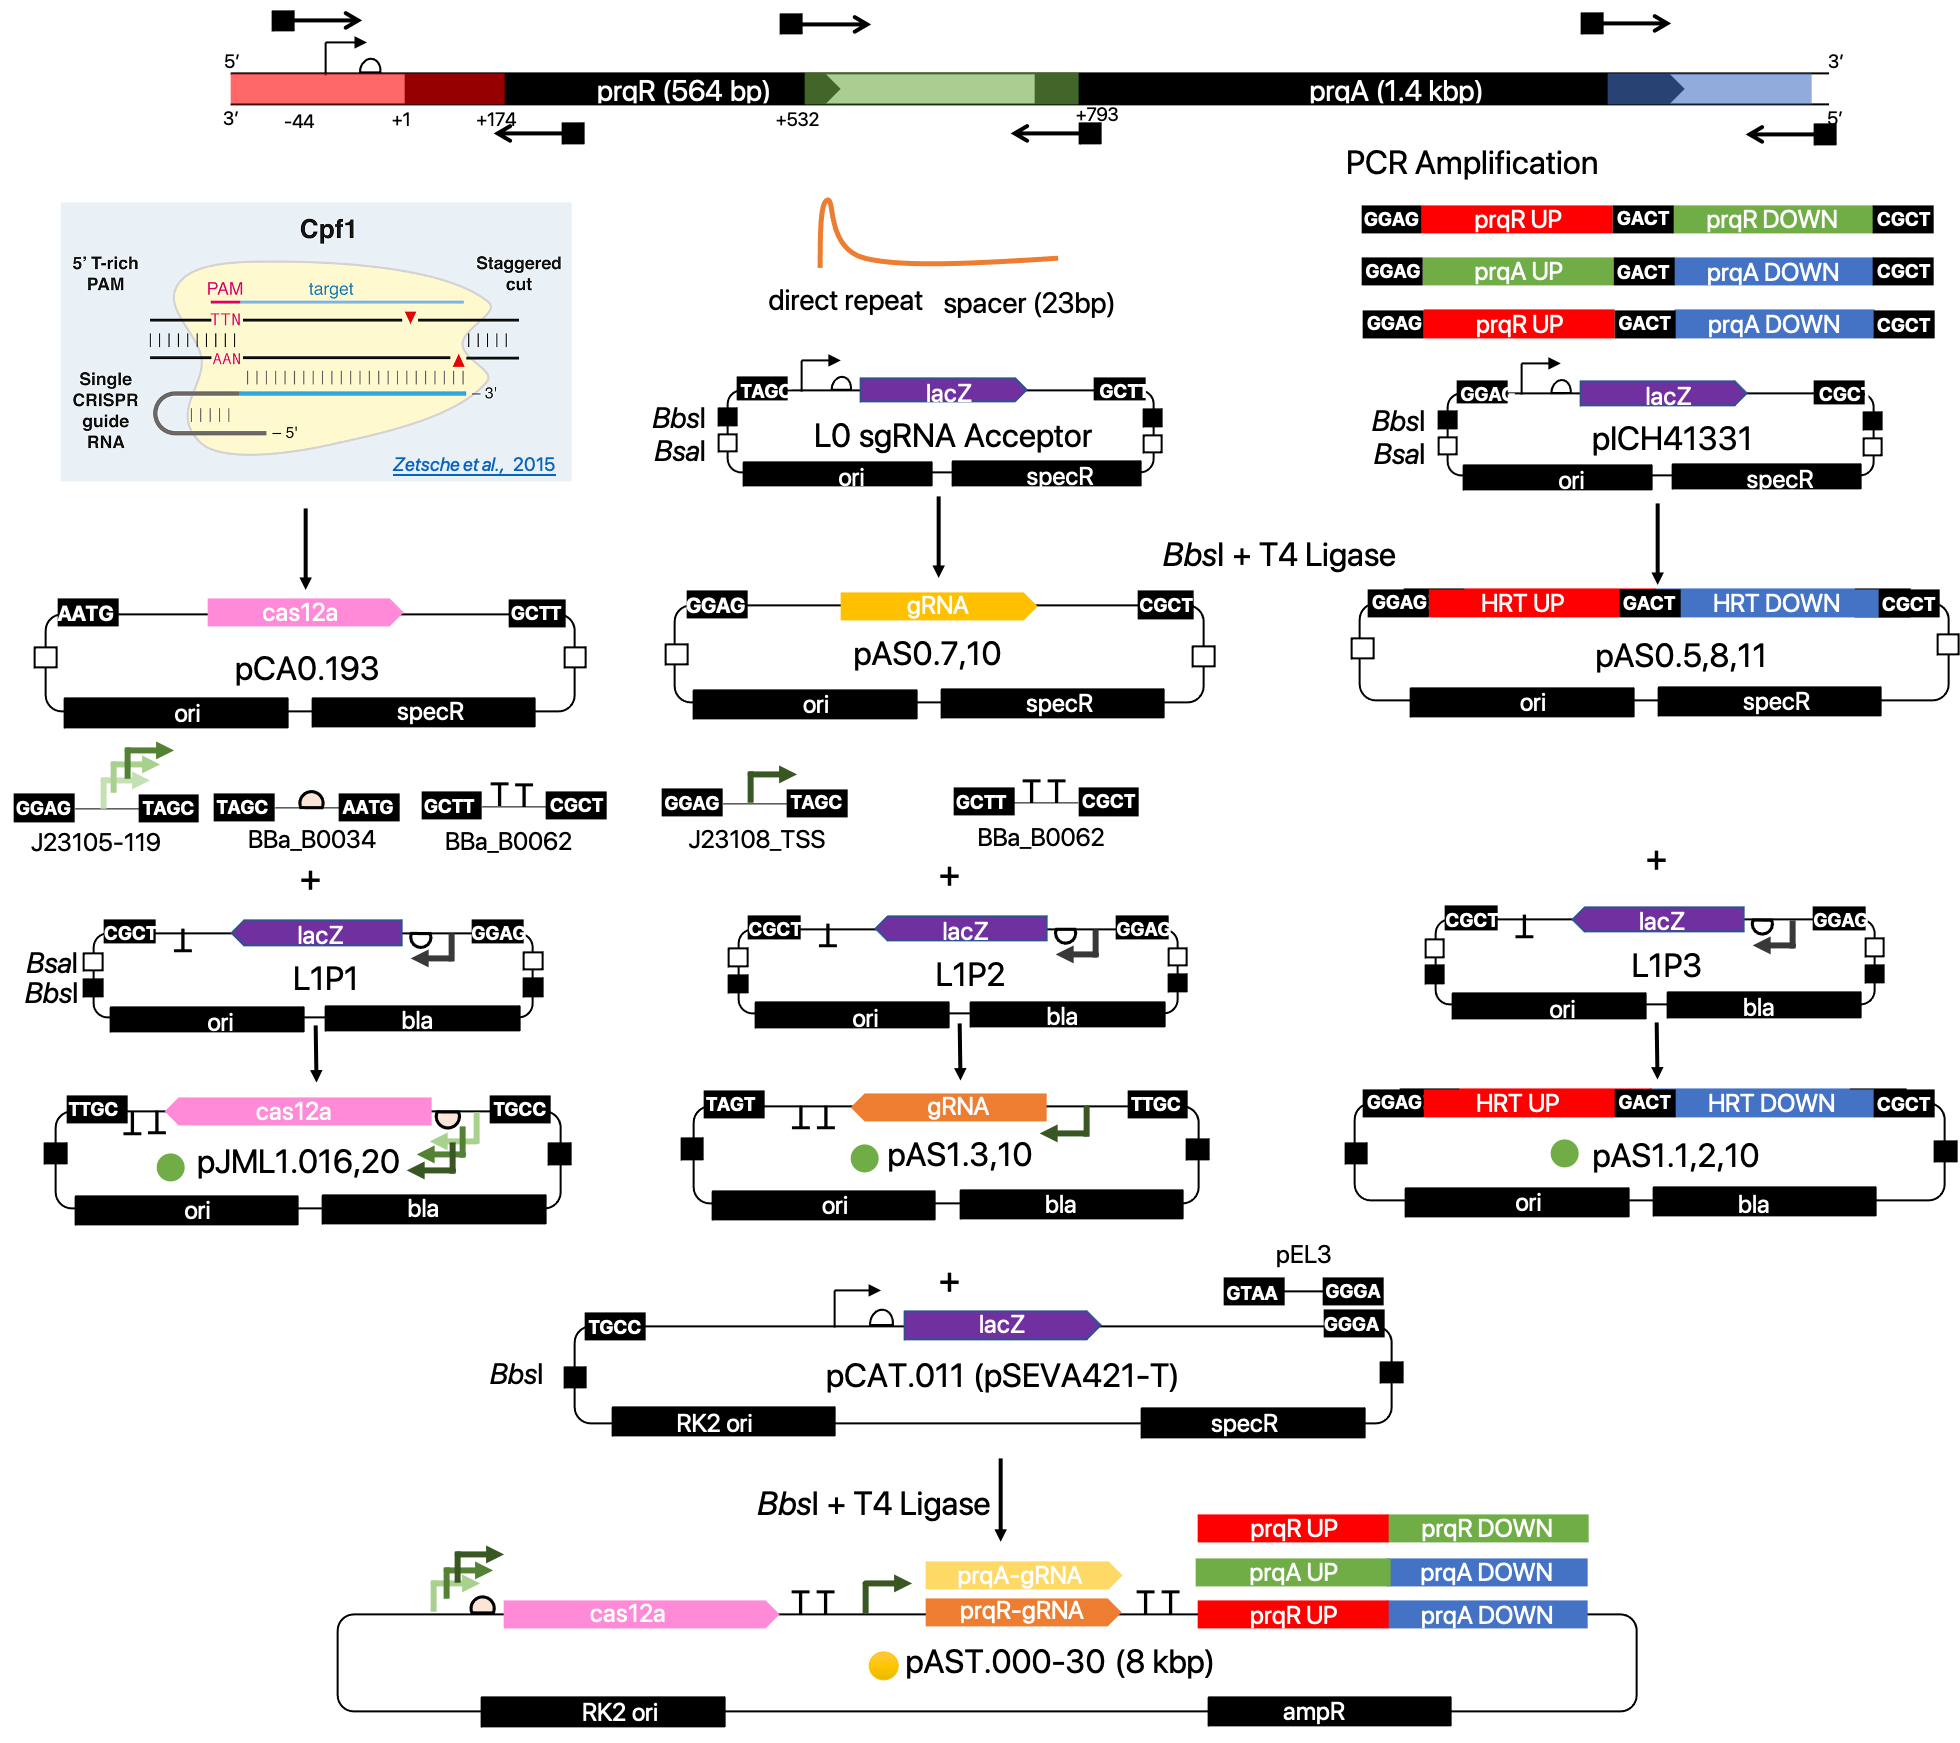
\includegraphics[width=\hsize]{figs/ASgate.png}
    \caption{Outline of the cloning strategy to construct modular knock-out plasmids. White and black squares indicate BbsI and BsaI recognition sites respectively. specR: spectinomycin resistance; bla: ampicillin/carbenicillin resistance; lacZ: beta-galactosidase coding sequence used for blue-white screening upon induction with IPTG and X-Gal.}
    \label{fig:KOstrategy}
\end{figure}

\newpage

\subsection{Level 0 Assembly}
To clone PCR products into MoClo acceptors. Restriction: BbsI; selection: spectinomycin.

\subsubsection{Homology Repair Templates}

\begin{figure}[H]
    \centering
    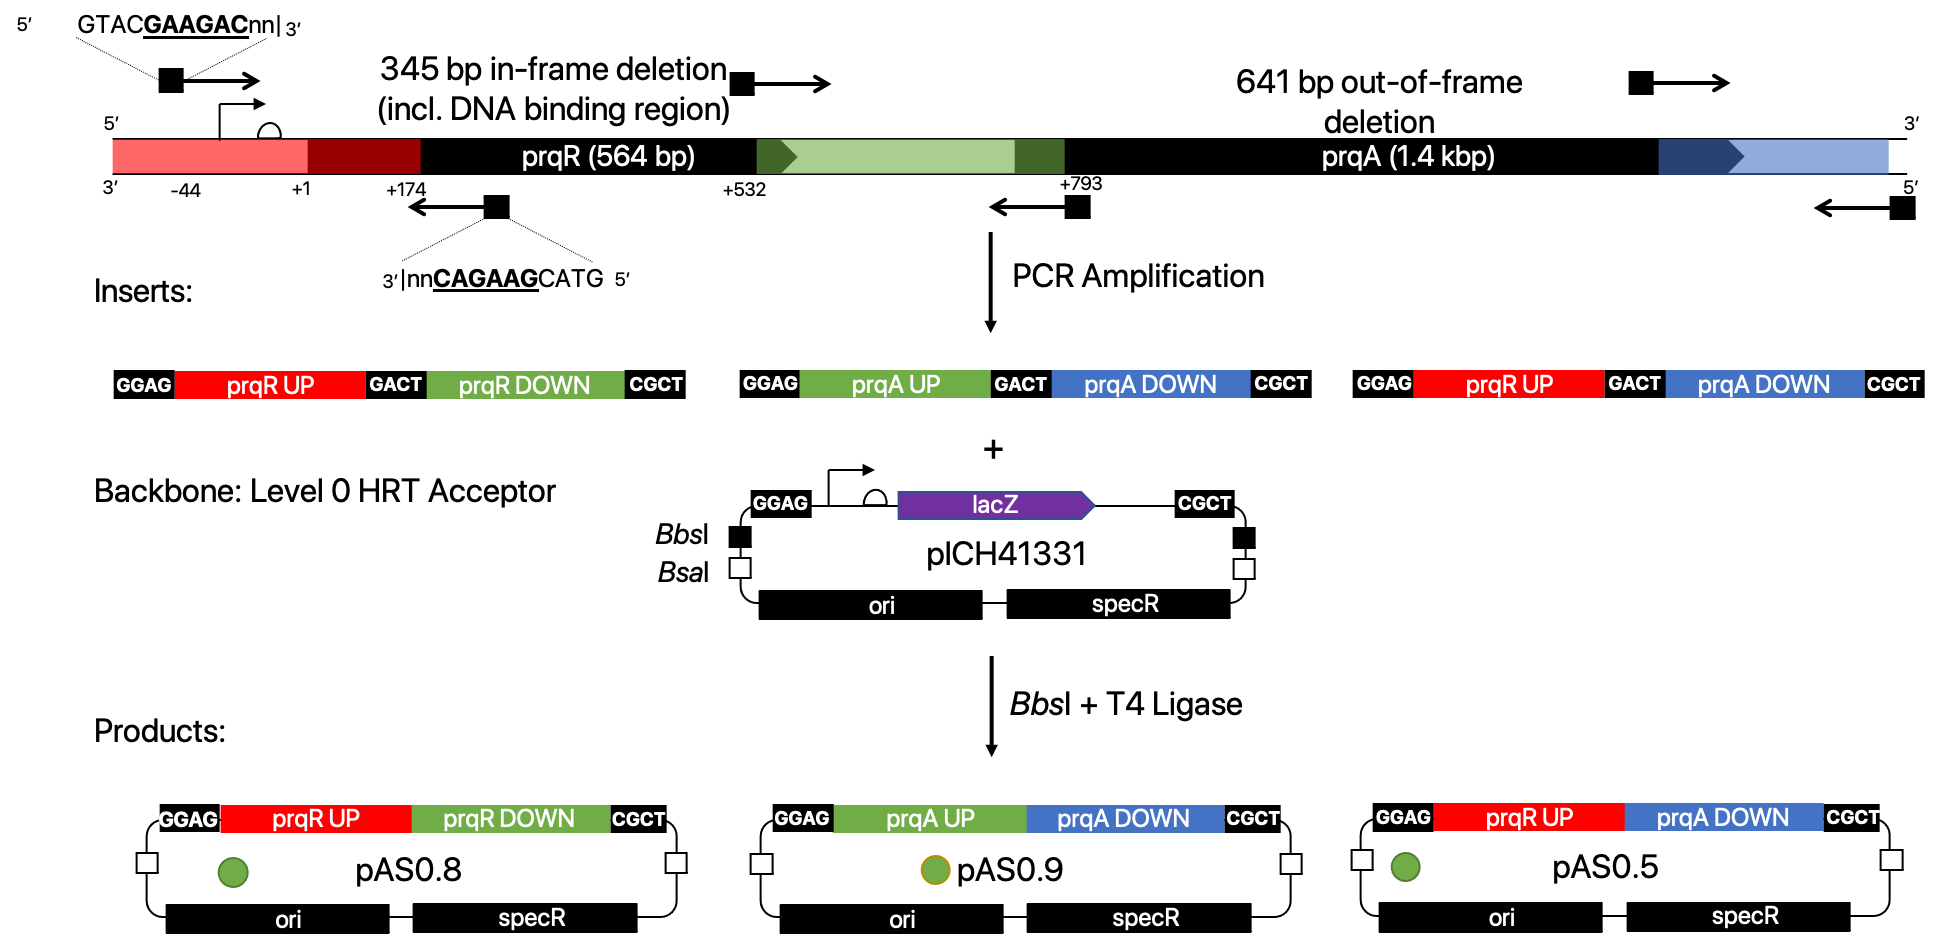
\includegraphics[width=\hsize]{figs/HRT.png}
    \caption{Cloning Homology Repair Templates into Level 0 Acceptors}
\end{figure}

\subsubsection{Coding Sequences}

\begin{figure}[H]
    \centering
    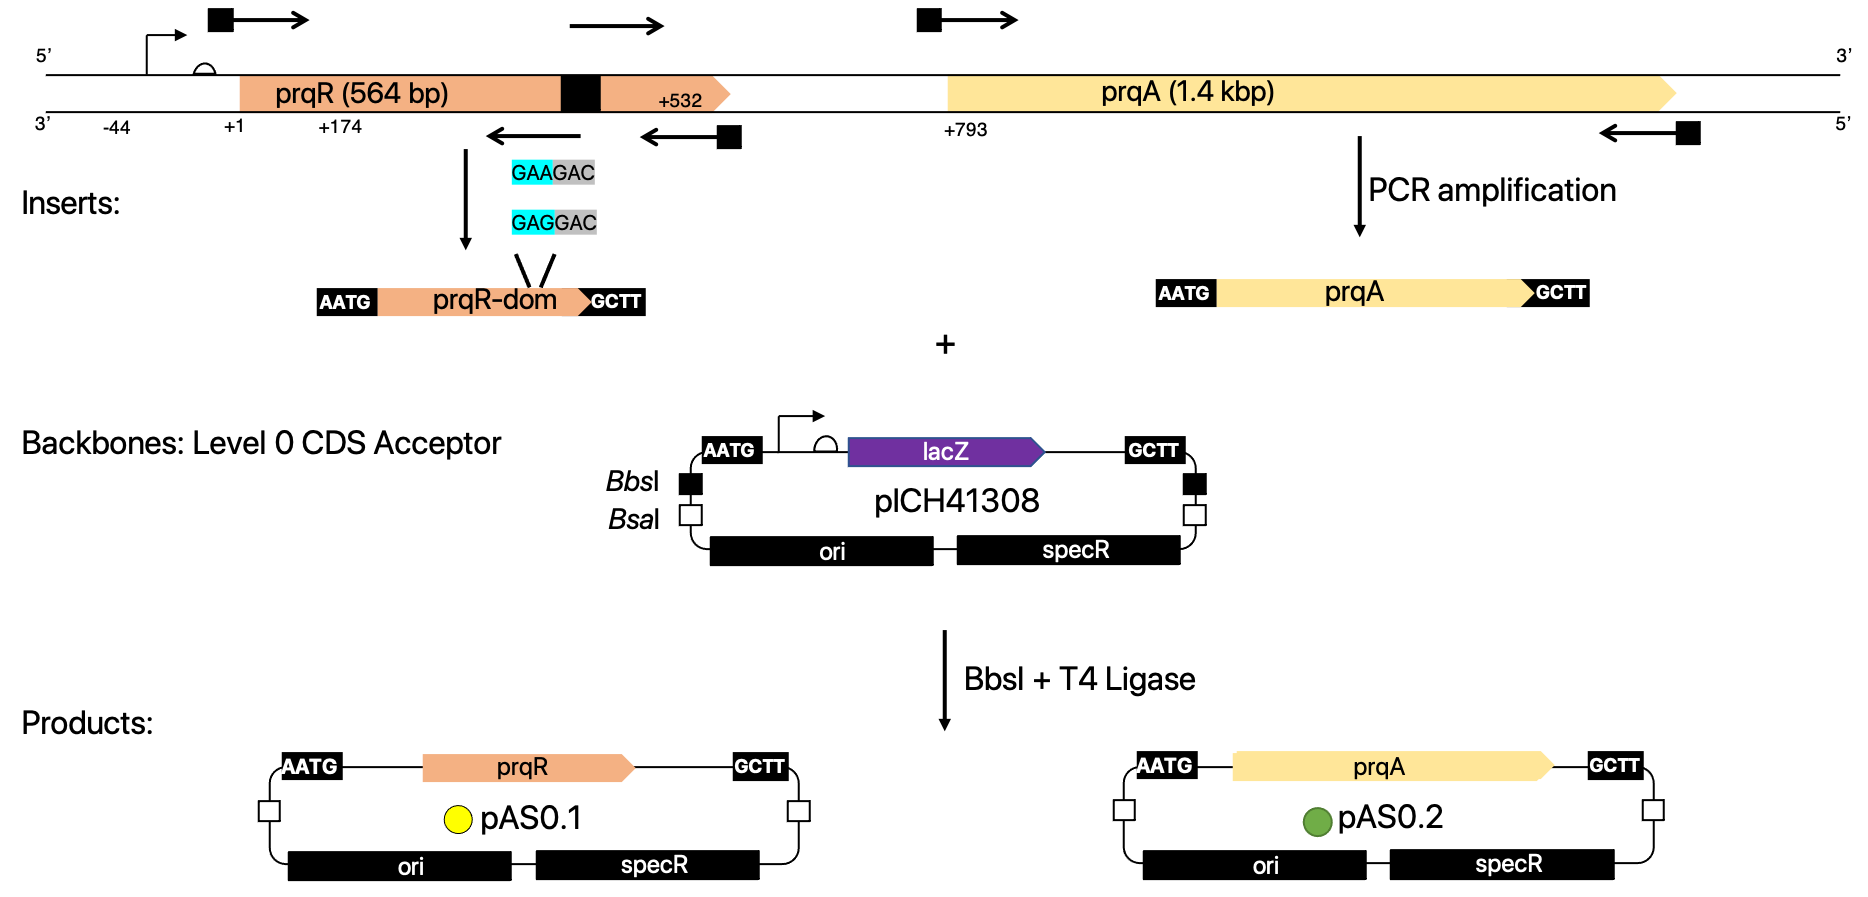
\includegraphics[width=\hsize]{figs/CDS.png}
    \caption{Cloning Coding Sequences into Level 0 Acceptors}
\end{figure}

\subsubsection{Cas12a gRNAs}

\begin{figure}[H]
    \centering
    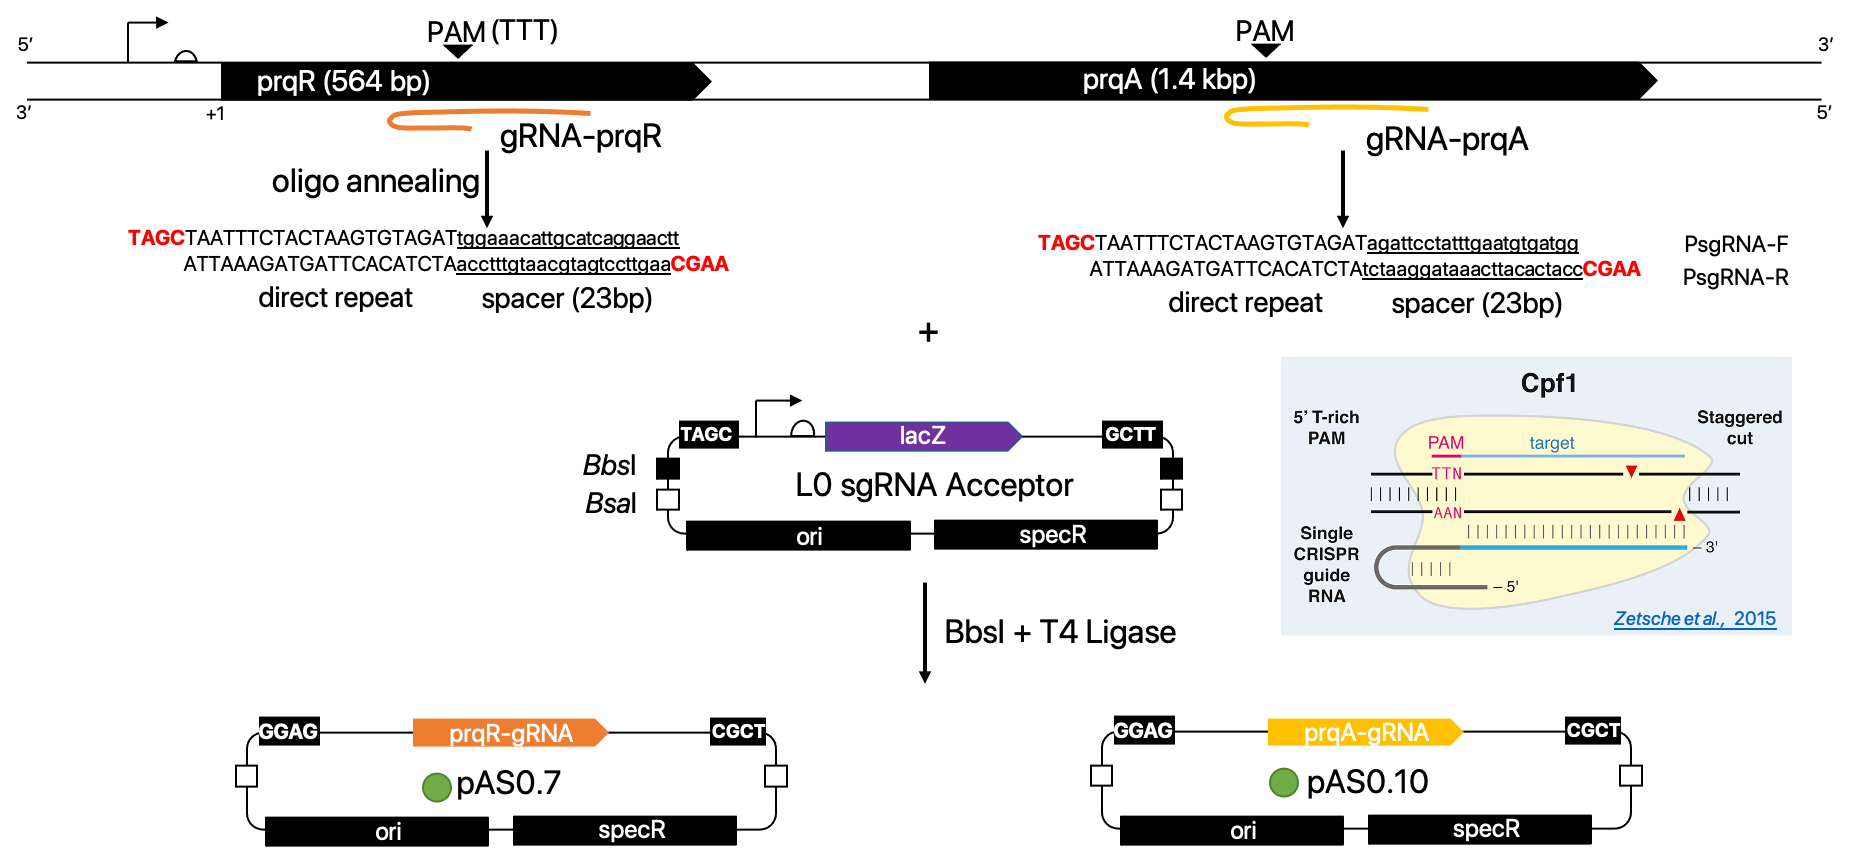
\includegraphics[width=\hsize]{figs/gRNA.png}
    \caption{Cloning Cas12a gRNA via oligo annealing into Level 0  acceptors}
\end{figure}
All the level 0 plasmids marked with a green dot has been validated by DNA sequencing. The coding sequence for the PrqR repressor contains a BbsI recognition site and still needs to be domesticated. Figure \ref{fig:L0} illustrates the library of DNA parts constructed during this project.
\begin{figure}[H]
    \centering
    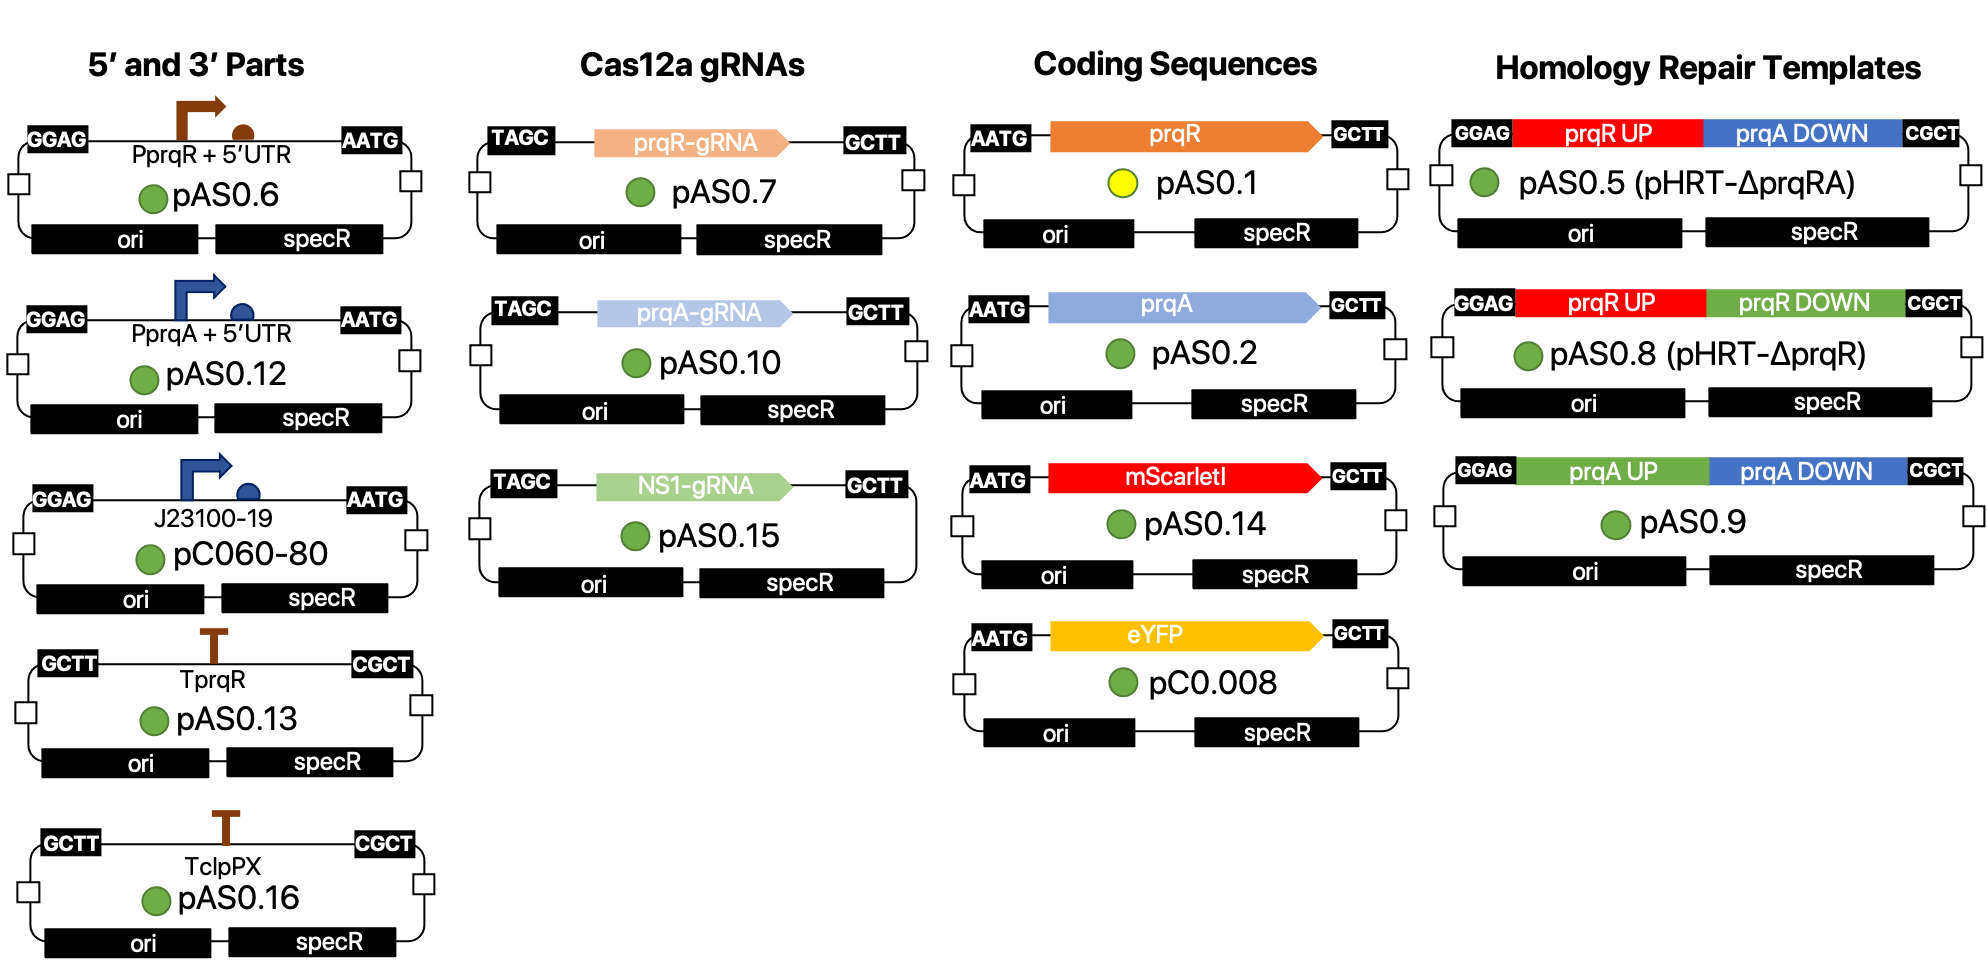
\includegraphics[width=\hsize]{figs/l0.png}
    \caption{Summary of level 0 library of plasmids assembled until now. Green dots indicate DNA parts validated by DNA sequencing. The pAS0.1 plasmid (yellow circle) contains an undesired mutation that still needs to be domesticated.}
    \label{fig:L0}
\end{figure}

\subsubsection{Level 1 Assembly}
Level 1 assembly reactions consist in cloning the inserts contained in level 0 plasmids into level 1 acceptor backbones. During this assembly reaction, the orientation of the level 0 parts will be inversed (genes will be in the reverse strand). This is not a problem as they will be reinverted in the next level T assembly reactions.
The CyanoGate level 1 acceptors are derived from the PlantGate MoClo toolbox. There are up to 7 different level 1 acceptors (L1P1, L1P2, ..., L1P7), which specify the position of level 1 expression units for multigene assembly into the final level T plasmids. For example, if the final plasmid requires two expression cassettes, one upstream of the other, the first unit will need to be cloned in L1P1, whilst the second one in L1P2. After level T assembly, the two cassettes will be found one after the other (separated by a 4 bp scar), in the forward strand in the level T plasmid. 


\begin{figure}[H]
    \centering
    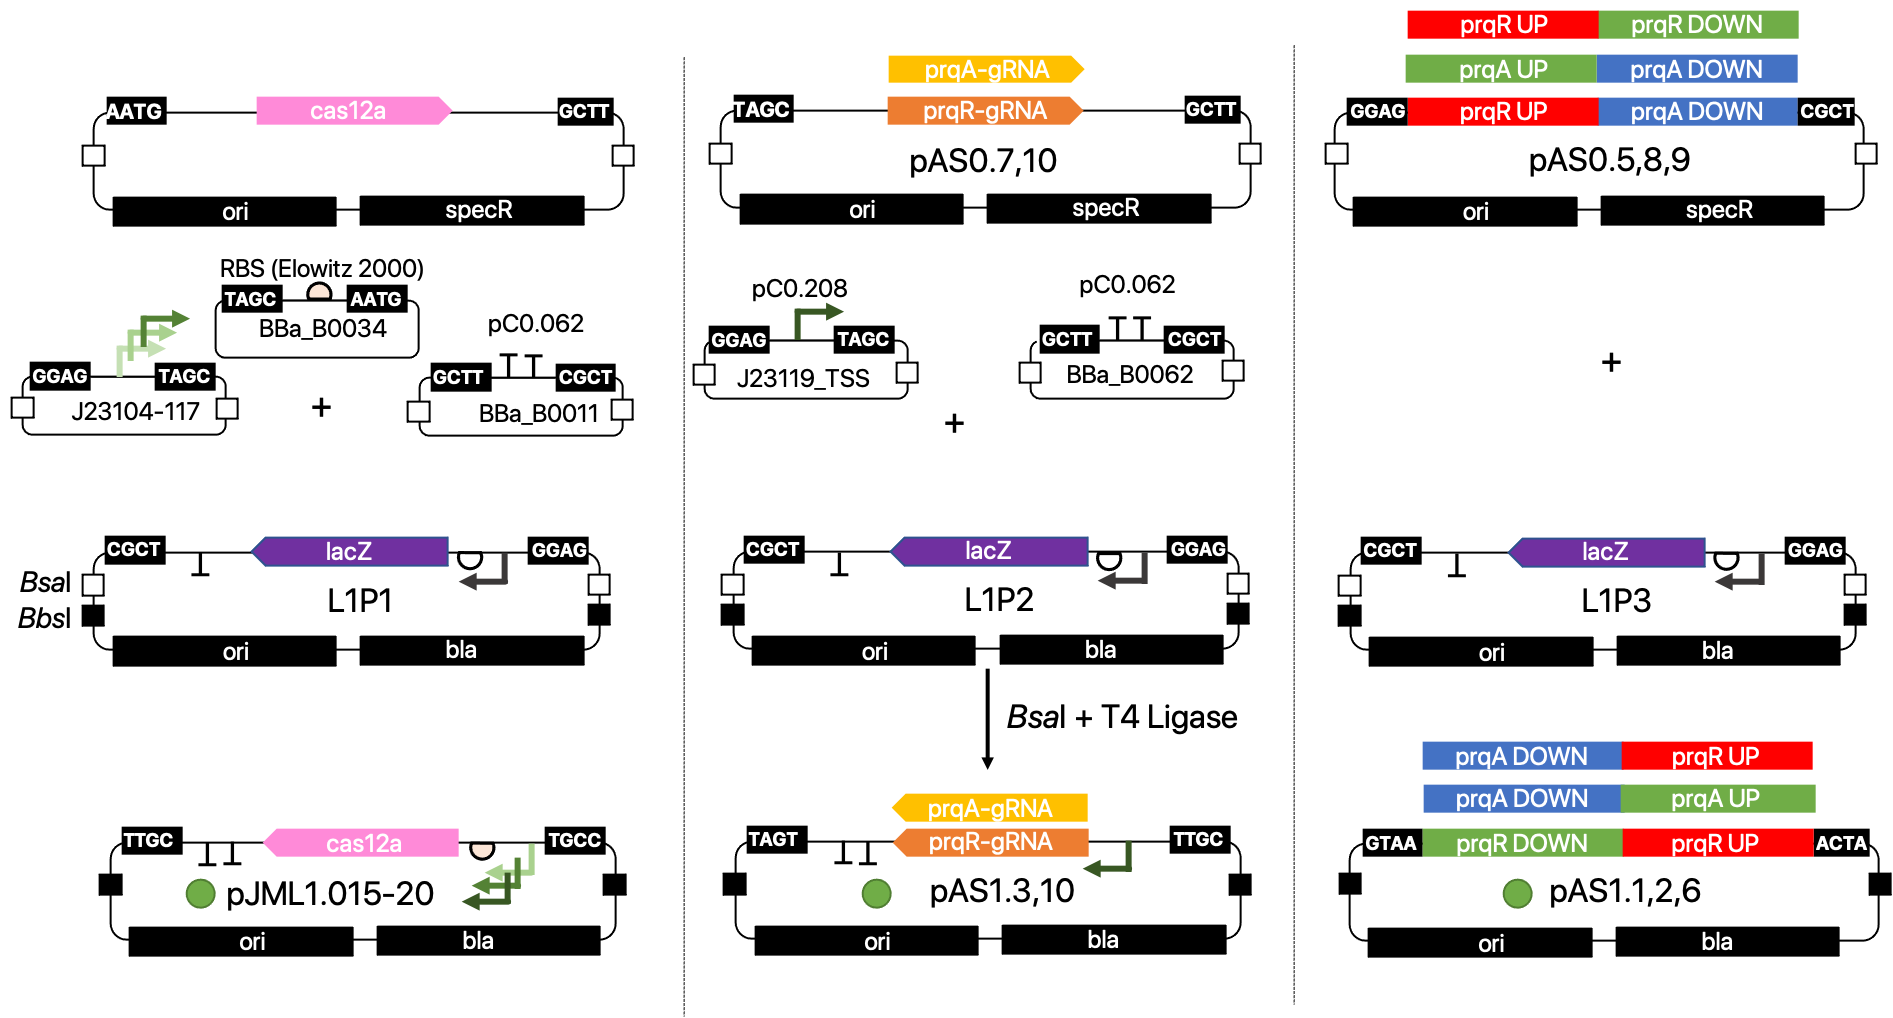
\includegraphics[width=\hsize]{figs/l1.png}
    \caption{Overview of the level 1 plasmids designed and assembled in this project.}
\end{figure}

\subsubsection{Level T Assembly}
Level T assembly consists in cloning multigene constructs from level 1 expression cassettes into level T acceptor backbones. Level T acceptors are shuttle vectors that replicate both in \textit{E. coli} and in a range of cyanobacteria hosts. This assembly step is performed with BbsI for restriction digestion. Selection depends on the antibiotic resistance gene encoded in the level T backbone. For the pCAT.011 (pSEVA421-T) backbone plasmid used in this study, spectinomycin was used as positive selection.
This plasmid is a MoClo-compatible vector derived from pSEVA421 and carries the RK2 replicative origin and has an average copy number of $\approx$ 10 in \textit{Synechocystis} \citep{Vasudevan2019}.

\subsubsection{Cloning level 1 parts into level T acceptors}
\begin{figure}[H]
    \centering
    \includegraphics[width=\hsize]{figs/LT.png}
    \caption{Cloning Level 1 into Level T Acceptors. SPT are sequencing primers designed to span the entire insert sequence for Sanger DNA sequencing.}
\end{figure}


\begin{figure}[H]
    \centering
    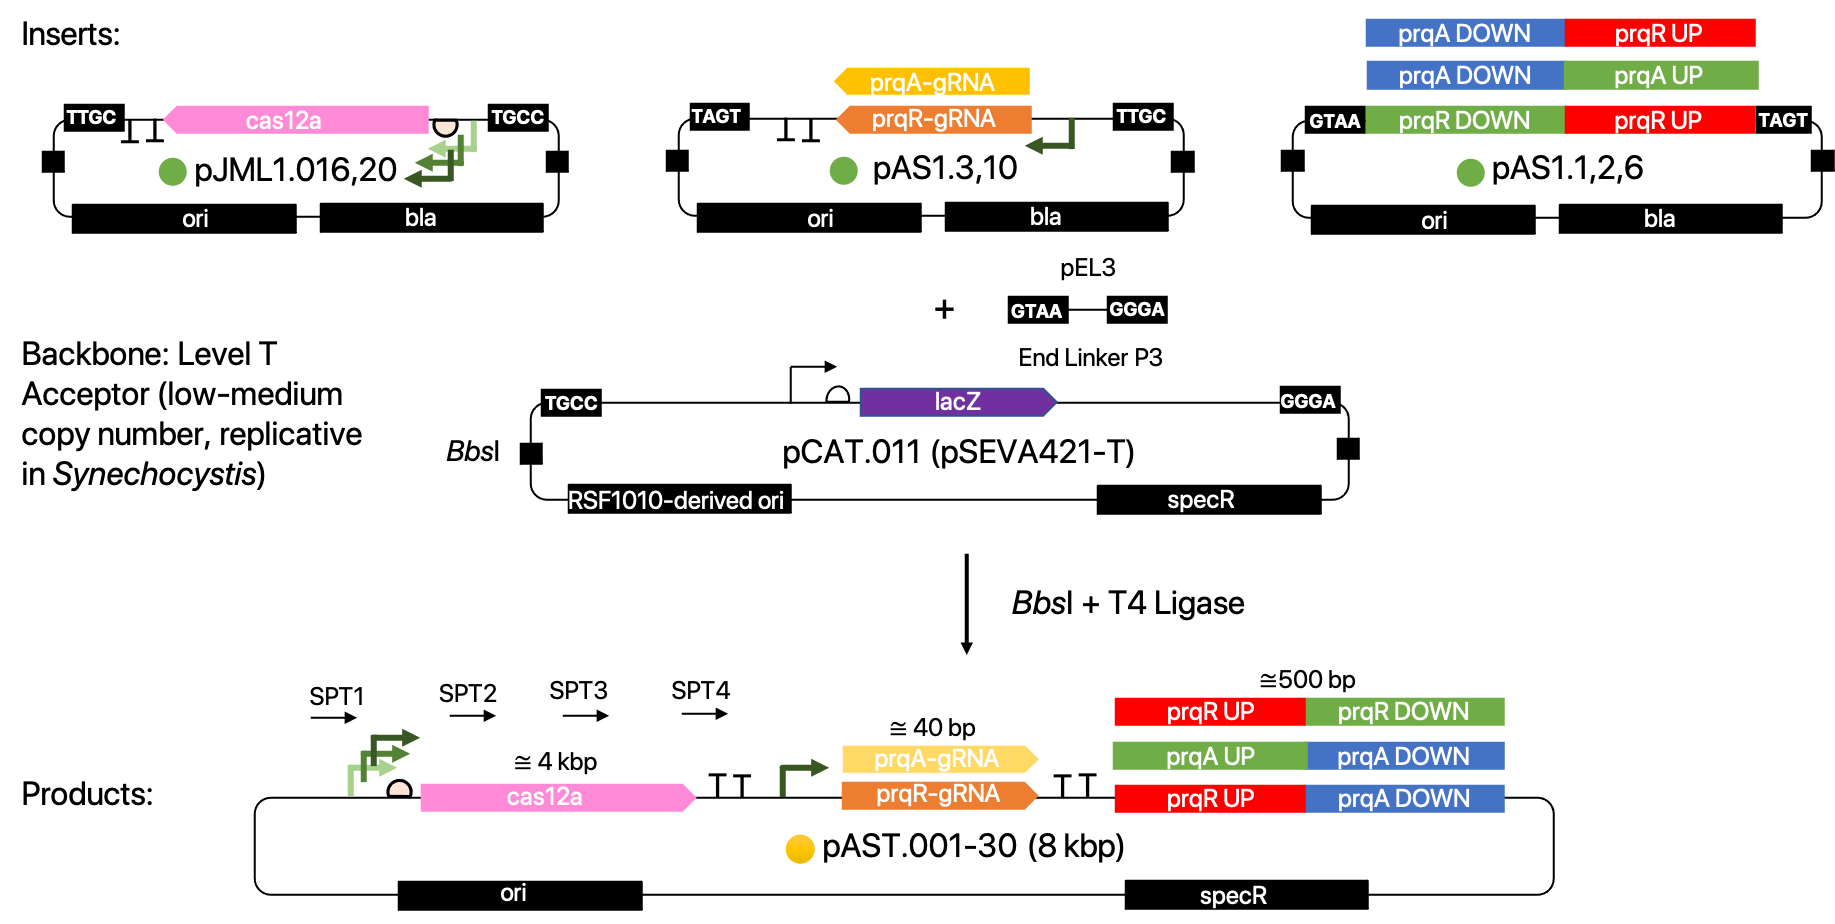
\includegraphics[width=\hsize]{figs/lt.png}
    \caption{Overview of level T plasmids designed and assembled in this project}
\end{figure}

\section{Construction of Fluorescent Reporter Plasmids}
In order to quantify the expression dynamics from native genes, a common approach in synthetic biology is to construct synthetic gene circuits by rewiring the  transcription factors and promoters to create novel regulatory topologies \citep{Chen2018}. During this project, the native PrqR transcription factor and the P$_{prqR}$ promoter have been used to construct synthetic gene circuits containing fluorescent reporter proteins regulated by these regulatory sequence.
To do so, the P$_{prqR}$ promoter sequence had to be annotated in the genome of \textit{Synechocystis sp.} PCC 6803. This was performed by identifying the DNA sequence extending 100 bp upstream of the first A nucleotide in the start codon (ATG) of the prqR gene. As shown in Fig. \ref{fig:promoteranal}, this sequence was aligned for comparison with the J23119 promoter sequence (which is a consensus eubacterial promoter commonly used as reference in synthetic biology). Using promoter and RBS prediction softwares (\href{http://www.bacpp.bioinfoucs.com/home}{BacPP}, \href{https://salislab.net/software/}{RBS calculator}), it was possible to identify certain features in the promoter sequence, such as the ribosome binding sites (RBS in green), the -10 and -35 regions (in yellow and purple, the sequences bound by the RNA polymerase sigma factors). The operator sequences (regions bound by repressor PrqR) were previously annotated by \citep{Babykin2003}.

\begin{figure}[H]
    \centering
    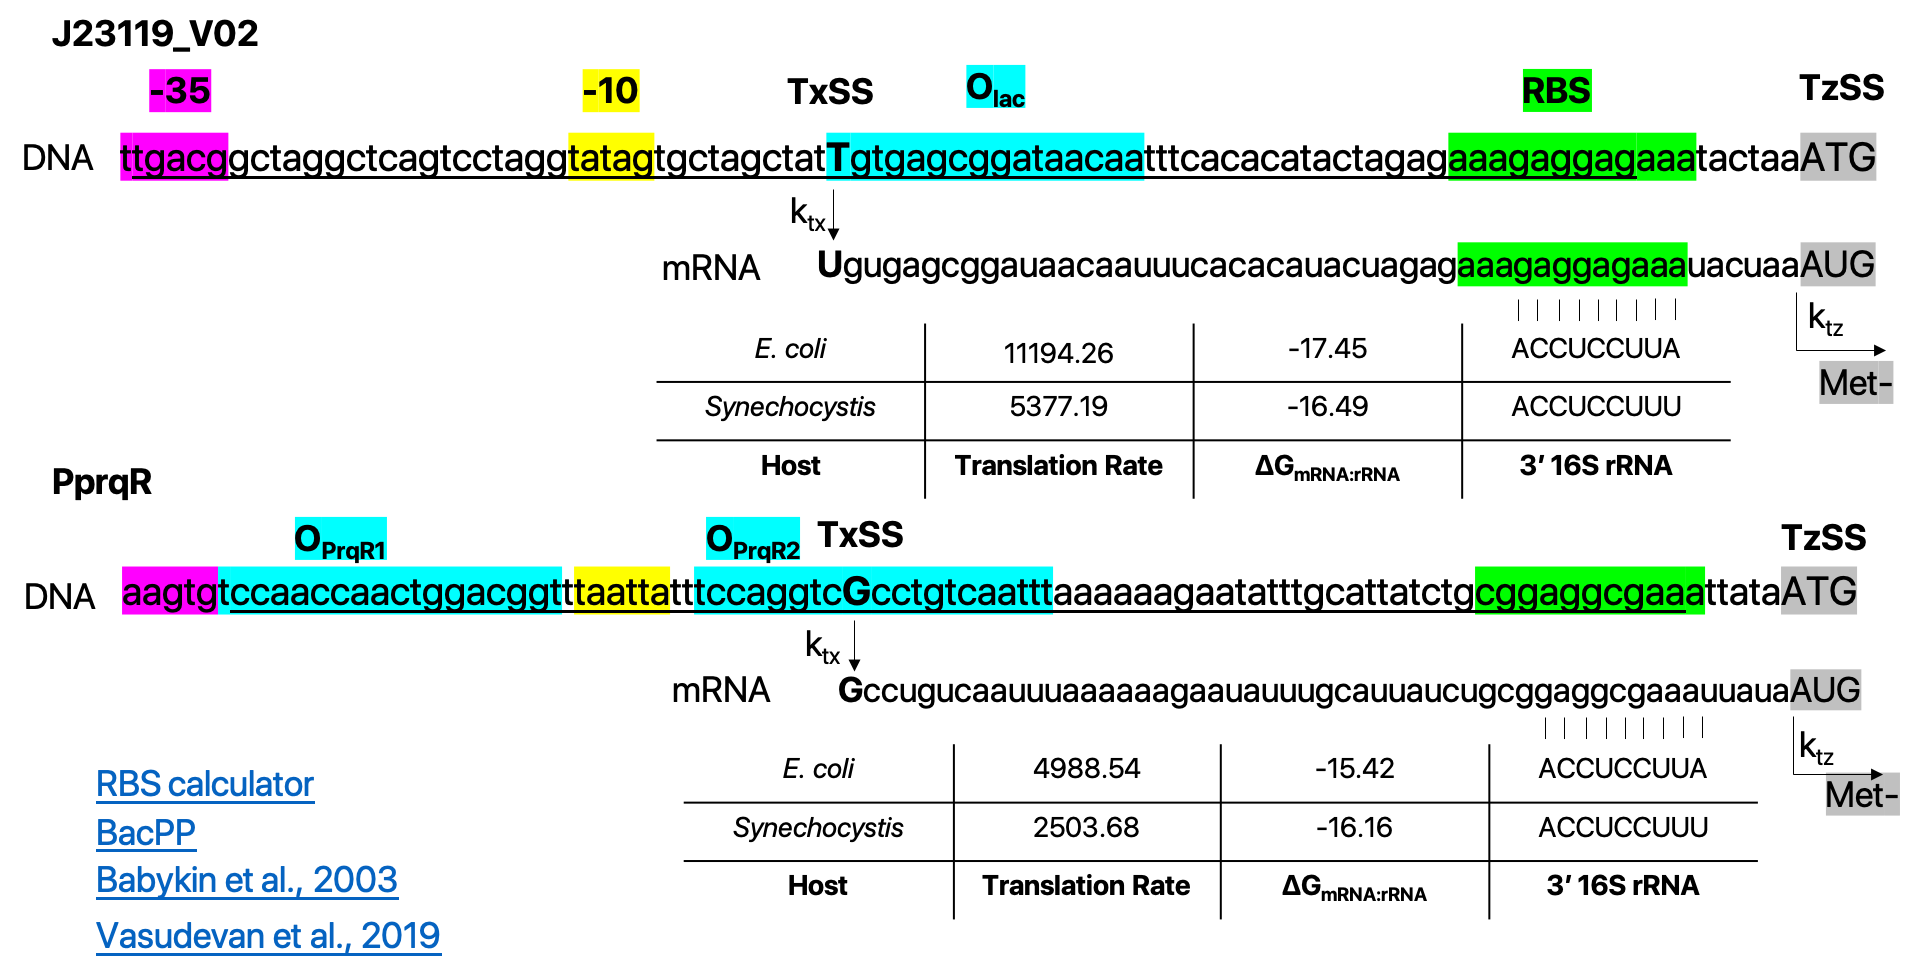
\includegraphics[width=\hsize]{figs/promoters.png}
    \caption{Comparison of the $P_{prqR}$ and the consensus J23119 promoter.}
    \label{fig:promoteranal}
\end{figure}

Cyanobacterial promoters can be categorised into three groups based on their sequences and which sigma factors recognise them. Type I promoters (recognised by $\sigma$70) contain both a −10 element (consensus 5’-TATAAT-3’) and a −35 element (consensus 5’-TTGACA-3’). Type II promoters contain the −10 element but lack a −35 element, instead containing operator sites bound by transcription factors. Type III promoters lack −10 or −35 elements and generally respond to various stresses through binding of type III sigma factors \citep{Gordon2018}.
Bioinformatic analysis of the $P_{prqR}$ promoter suggested that this promoter might be a type II promoter. In fact it contains a −10 element but the sequence at the −35 location is quite dissimilar to the -35 consensus (5’-TTGACA-3’), and instead contains two operator sites recognised by its repressor PrqR.

After this analysis, the annotated P$_{prqR}$ promoter sequence was assembled from annealing and extension of a pair of oligos (P58 and P59 in Table \ref{table:primers}) with overhangs compatible with the level 0 promoters acceptor.
This sequence was cloned upstream of the fluorescent protein eYFP. A positive control was constructed by replacing the P$_{prqR}$ with the J23119 consensus promoter. Terminators (T$_{clpPX}$) were added at the 3' end. 
The protein eYFP was chosen because of its fluorescent signal orthogonal to to the endogenous background fluorescence of \textit{Synechocystis sp.} PCC 6803 (Fig. \ref{fig:fluo}).

\begin{figure}[H]
    \centering
    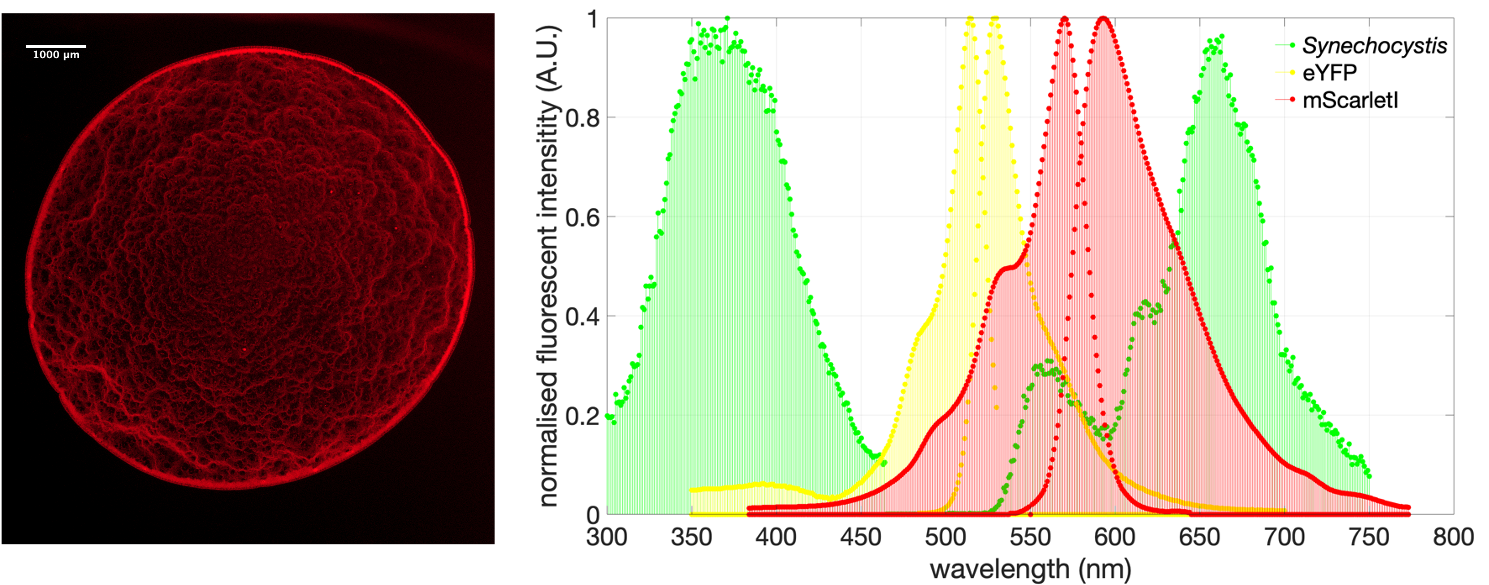
\includegraphics[width=\hsize]{figs/fspectracells.png}
    \caption{On the left: A colony of $\approx$ 4 million WT \textit{Synechocystis sp.} cells visualised under a fluorescence microscope ($\lambda_{em} = 667 nm$). The red signal is the endogenous fluorescence emitted by photosynthetic components (e.g. chlorophylls). On the right: fluorescence spectra of whole cells overlayed with those of the fluorescent reporters eYFP (yellow) and mScarlet-I.}
    \label{fig:fluo}
\end{figure}

\section{Mathematical Modelling of PrqR Dynamics}

The synthetic negative feedback network displayed by the prqRA operon was formalised using mathematical modelling in MATLAB R2019b. Regulation at both the transcriptional (repressor-promoter) and translational levels was modelled using a simple system of ordinary differential equations (ODE) commonly used to predict expression kinetics of synthetic gene circuits.
The autorepressor was simulated using a two-state model similar to previously described models of the TetR autorepressor (\citealt{Braun}; \citealt{Kelly2018}). The aim of this modelling is to predict the fluorescence output from the reporter plasmids constructed in this study depending on the concentration of redox-mediator. In one direction (theory $\rightarrow$ experiments), these results can help to identify suitable ranges of concentration of redox mediators to capture the sigmoidal fluorescence output characteristic of inducible promoters. In the other direction (experiments $\rightarrow$ theory), using this theoretical framework it would be possible to estimate the concentration of ligand effector present in the cell given the fluorescence output quantified from the experiments.




\begin{figure}[H]
    \centering
    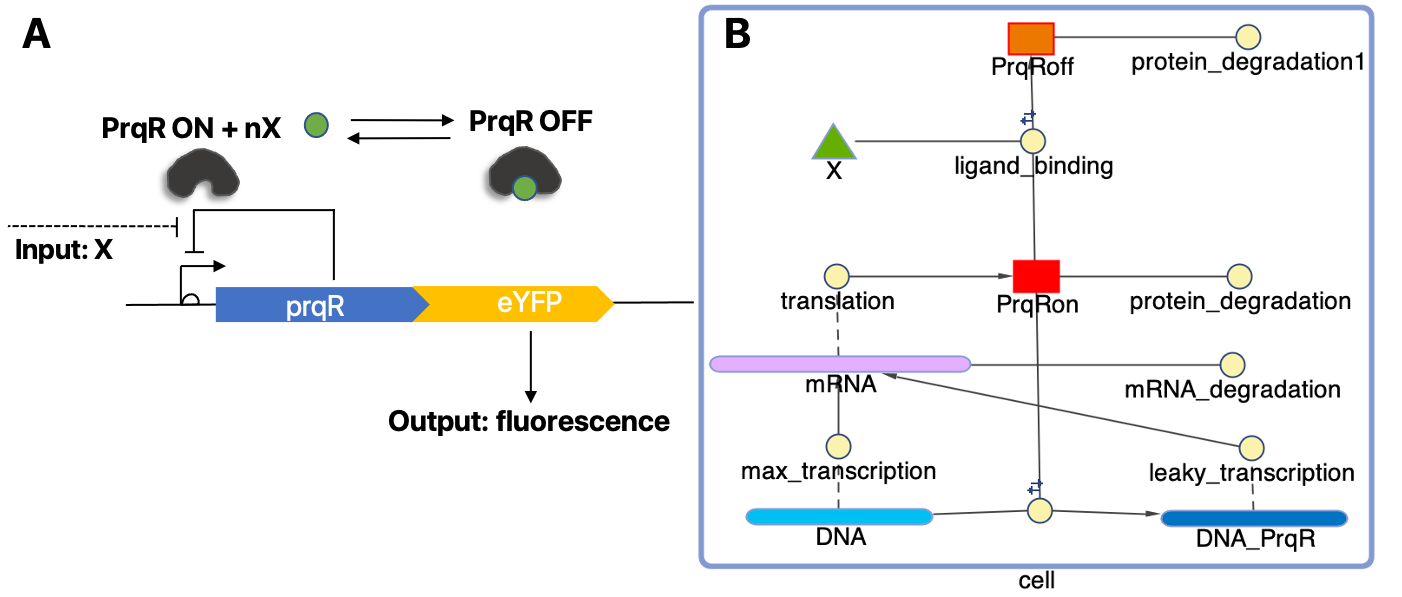
\includegraphics[width=\hsize]{figs/modelling.png}
    \caption{Schematic overview of a simple ODE model to simulate dynamics of prqRA operon. The PrqR repressor is an autorepressor of its own P$_{prqR}$ promoter. It has been assumed that the PrqR repressor behaves as other repressor in the tetR-like family. These transcriptional regulators generally exist in two states (ON or OFF) depending on the presence of ligand molecules. In the ON state, they represses transcription from their cis-regulatory sequences (e.g. prqR and eYFP in this case). Binding with ligand X induces a conformational change in the DNA-binding domain of the repressor, resulting in its inactivation (OFF) and consequent transcription of prqR and eYFP genes.}
\end{figure}

\subsection{Modelling Gene Expression}
Gene expression dynamics for the PrqR-YFP device is modelled with a simple system of kinetic reactions depending on two states: the concentration of mRNA (r) and protein (R). The underlying biochemical reactions (transcription, translation, degradation) can be expressed as:

\begin{equation}
\begin{gathered}    
    \emptyset \xrightarrow{k_{tx}} r \xrightarrow{d} \emptyset\\
    r \xrightarrow{k_{tz}} r + R\\ 
    R \xrightarrow{D} \emptyset
\end{gathered}
\end{equation}
Where $\Theta$ indicate empty sets (genes, degradation), $k_{tx}$is the apparent transcription rate, d is the mRNA degradation rate, $k_{tz}$ is the translation rate and D is the protein degradation rate. These reactions are described by two sets of ODEs:

\begin{equation}
\label{eq:transcription1}
    \frac{\delta r}{\delta t} = k_{tx}r - dr
\end{equation}

\begin{equation}
    \frac{\delta R}{\delta t} = k_{tz}r - DR
\end{equation}

\subsection{Repressor and Ligand Binding}
The binding between repressor and ligand is modelled as a second-order kinetic reaction. The DNA-bound active repressor, $R_{on}$, reacts with ligand X to form the inactive form of the repressor-ligand complex, $R_{off}$:
\begin{equation}
   R_{on} + nX \stackrel[k_{r}]{k_{f}}{\leftrightarrows} R_{off} 
\end{equation}
where n is the number of ligand binding sites in R,  $k_{f}$ and $k_{r}$ are the forward and reverse reaction rates. The rate of appearance of the repressor-ligand complex can then be described by the following ODE

\begin{equation}
\label{eq:ligandbinding}
    \frac{R_{off}}{dt} = k_{f}[R_{on}][X]^{n} - k_{r}[R_{off}] 
\end{equation}

If $[R_{off}]$ is initially zero, the concentrations will shift until the forward reaction rate is equal to the reverse reaction rate, such that the concentrations no longer vary with time. At this equilibrium point, the concentration of the complex won’t vary with time. Therefore equating Equation \ref{eq:ligandbinding} to 0 and after some algebraic rearrangement, the fractions of bound repressor molecules as a function of ligand concentration are described by the following Hill equation:

\begin{equation}
\label{eq:Hill}
    \Theta = \frac{Bound [PrqR]}{Total [PrqR]} =  \frac{[R_{off}]}{[R_{on}] + [X]^{n}}
\end{equation}

Therefore multiplying the total PrqR concentration, R, with the fraction of unbound molecules (1-$\Theta$) enables to calculate the concentration of active (DNA-bound) repressors at steady state:

\begin{equation}
\label{eq:Ron}
	R_{on} = R\cdot(1-\Theta) = R\cdot(1 - \frac{[X]^n}{Kd_{x} + [X]^n})
\end{equation}

Where  Kd$_{x}$  is the apparent dissociation constant, defined as the ratio of the dissociation rate constant ($k_{r}$) and the association rate constant ($k_{f}$) such that:

\begin{equation}
	Kd_{x} = \frac{k_{r}}{k_{f}} = \frac{[R_{on}][X]^n}{[R_{off}]}
\end{equation}

\subsection{Transcription as a Function of Active Repressor}
Equation \ref{eq:transcription1} describes the rate of transcription from the P$_{prqR}$ promoter but assumes that the promoter is very strong, such that all promoters were bound. However, in the case of prqR-mediated autorepression, we need to account for the amound of promoter sites bound by the repressor. It is assumed that all the repressors unbound by the ligand will bind to the promoters and vice versa.  Using the hill equation (Equation \ref{eq:Hill}), it is possible to describe the transcription from the P$_{prqR}$ promoter as a function of the concentration of active repressors, with the generic equation of the form:

\begin{equation}
\label{eq:transrep2}
    \frac{\delta r}{\delta t} = k_{tx} \cdot (1 - \frac{[R_{on}]^{N}}{K_D + [R_{on}]^{N}}) = \frac{k_{tx}}{1 + \frac{[R_{on}]^N}{K_D}}
\end{equation}

Additionally, even when fully bound, the promoter is still able to transcribe the downstream gene, but at a reduced rate. This is described as leaky transcription. The maximum transcription rate, $K_{tx}$ is therefore redefined as $\alpha$ + $\alpha_{0}$ in the presence of no repressors bound to the promoter and $\alpha_{0}$ when saturated with repressor R. The change in concentration of mRNA over time as a function of the repressor bound to the promoters can be then rewritten as:
    
\begin{equation}
    \frac{\delta r}{\delta t} = \frac{\alpha}{1 + \frac{[R_{on}]^{N}}{K_D}} + \alpha_{0}
\end{equation}

\subsection{Final System of ODEs}
By substituting the concentration of active repressor calculated in Equation \ref{eq:Ron} with $R_{on}$ of Equation \ref{eq:transrep2}, results in the final ODEs describing transcription of r as a function of ligand concentration: 
\begin{equation}
\label{eq:transcrtiptionrepress}
    \frac{\delta r}{\delta t} = \frac{\alpha}{1 + \frac{(R\cdot(1 - \frac{[X]^n}{Kd_{x} + [X]^n}))^{N}}{K_D}} + \alpha_{0} - dr
\end{equation}

The translation of r into R is given by Equation \ref{eq:translationtot}, which describes the change in protein concentration, R, over time as a function of the translation and degradation of mRNA,r.
\begin{equation}
\label{eq:translationtot}
    \frac{\delta R}{\delta t} = k_{tz}r - DR
\end{equation}


\subsection{Deterministic Simulation}
Equations \ref{eq:transcrtiptionrepress} and \ref{eq:translationtot} have been solved numerically using Matlab ode45 solver. The parameters used to run the simulation have been taken from biologically similar systems and are listed in Table \ref{table:params}. Future experimental efforts will also involve the quantification of some of these parameters.

\begin{table}[H]
\centering
\begin{tabular}{l|l|l|l|l}
\textbf{} & \textbf{Description} & \textbf{Value} & \textbf{Unit} & \textbf{Reference} \\ \hline
$\alpha$ & transcription rate of tetR-GFP gene from Ptet & 0.085 & nM $s^{-1}$ & \cite{Braun}\\ \hline
$\alpha_{0}$ & transcription leak rate of tetR-GFP gene from Ptet & 0.05 & nM $s^{-1}$ & \cite{Kelly2018} \\ \hline
d & mRNA degradation rate  & 4.1 $\cdot$ 10$^{−3}$ & s$^{-1}$  & \cite{Kelly2018}  \\ \hline
D & protein degradation rate & 3.9 $\cdot$ 10$^{−4}$ & s$^{-1}$  & \cite{Kelly2018}   \\ \hline
$k_{tz}$ & translation rate from from Ptet & 0.0154   & $s^{-1}$  & \cite{Kelly2018}  \\
\end{tabular}
\caption{List of parameters used utilised to simulate the system of ODEs}
\label{table:params}
\end{table}

As shown in Figure \ref{fig:modelgraphs} (on the left), the model predicts that the higher the concentration of inducer, the higher the steady-state fluorescence intensity. By plotting the steady state fluorescence as a function of ligand concentration, the model also predicts a sygmoidal dose response to the logarithm of ligand concentration. This is characteristic of a double-negative feedback with cooperativity \cite{Kelly2018}. The cooperativity parameter (the Hill coefficient n) determines the steepness of the response and can be fitted with experimental data to estimate the number of repressor monomers binding cooperatively to the promoter. These results have been simulated with parameters for the TetR repressor and tetracycline as the inducer. However, in the future, these parameters will be adapted to the ones for the redox-mediator tested experimentally (e.g. methyl viologen, pyocyanin etc...). The reporter devices will be characterised using serial dilutions of a range of different putative inducers. If the experimental data for a given inducer fit with the theoretical predictions of double-negative feedback, this would suggest that the inducer under study is a potential ligand to PrqR.

\begin{figure}[H]
    \centering
    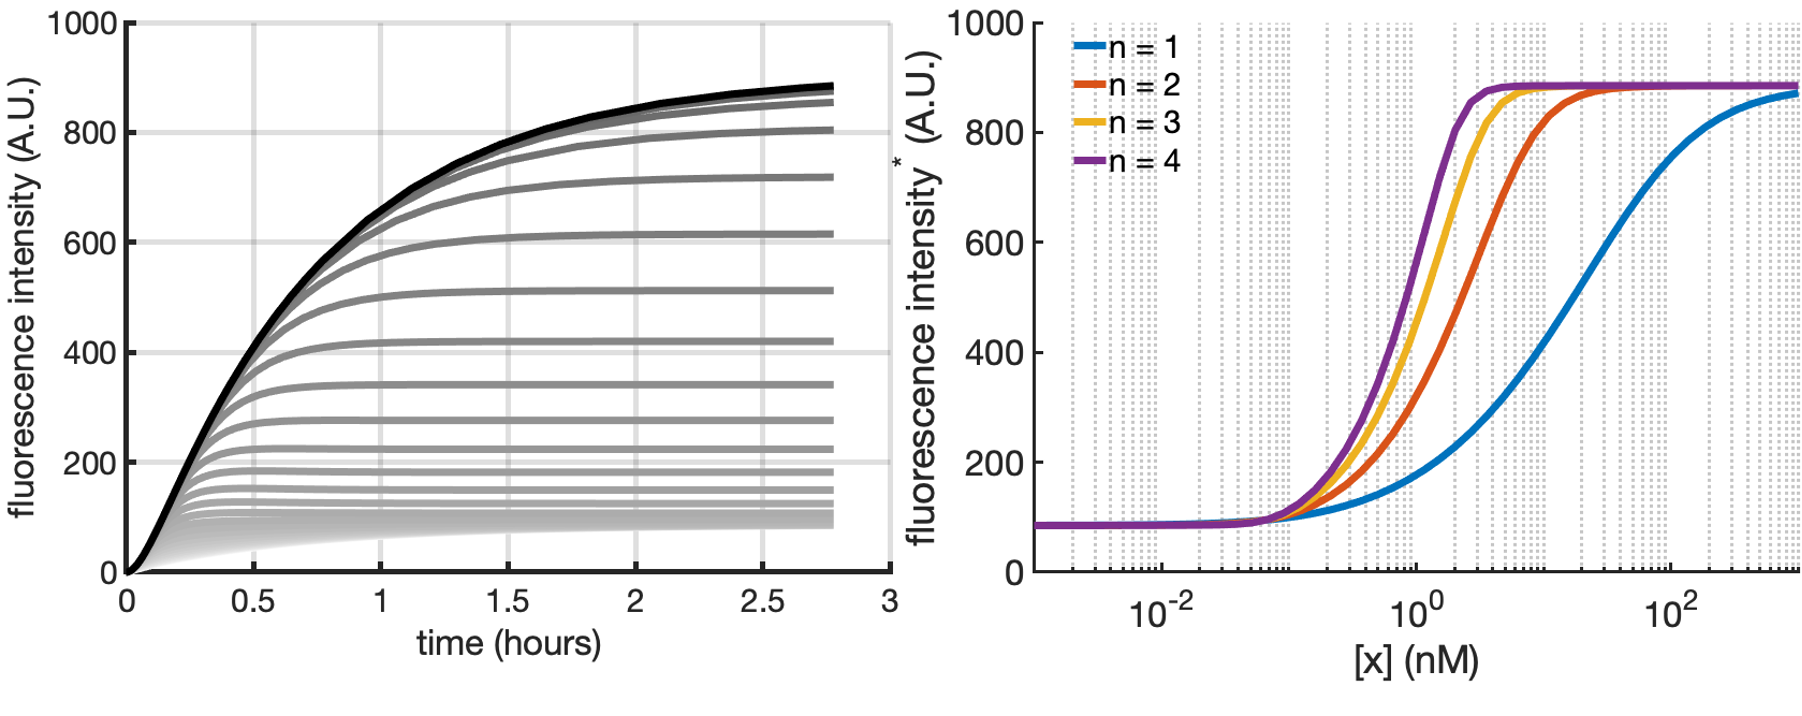
\includegraphics[width=\hsize]{figs/simulations.png}
    \caption{Numerical simulations of the system of ODEs describing the dynamics of PrqR regulation. On the left:eYFP fluorescence as a function of time for increasing concentrations of putative inducer X (increasing shades of grey). On the right: steady-state fluorescence response as a function of the logarithm of the inducer concentration. Lines of different colours indicate simulations with different Hill coefficients according to legend in the top left corner.}
    \label{fig:modelgraphs}
    \end{figure}
